\chapter{Studi Literatur}

Pada bab ini, Penulis akan menguraikan hasil literatur dalam penyusunan tugas
akhir ini. Subbab pertama membahas simulator CARLA, yaitu perangkat lunak yang
digunakan sebagai alat simulasi. Subbab kedua menjelaskan NVIDIA Pegasus yang
akan digunakan sebagai mesin untuk menjalankan algoritma \textit{decision
    making} di lingkungan simulasi dan \textit{production}. Lalu, pada subbab
ketiga akan dibahas beberapa cara komunikasi yang dapat digunakan pada sistem
terdistribusi. Terakhir, subbab keempat akan membahas penelitian-penelitian
terkait simulasi \textit{autonomous vehicle} menggunakan CARLA.

\section{Simulator CARLA}
\blindtext

% TODO: Masukin hubungan dengan NVIDIA Pegasus

\section{NVIDIA Pegasus}

NVIDIA Pegasus adalah salah satu produk cetusan NVIDIA Corporation di bawah
lini produk NVIDIA Drive PX. Nama pasar dari NVIDIA Pegasus adalah NVIDIA Drive
PX Pegasus. Lini produk NVIDIA Drive sendiri merupakan platform komputer untuk
memberikan fungsionalitas bantuan mengemudi pada kendaraan bermotor.

\begin{figure}
    \begin{center}
        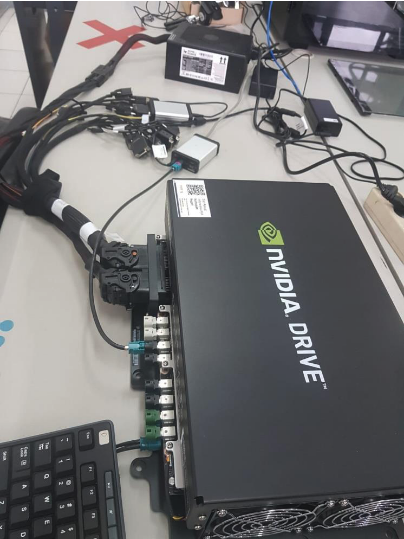
\includegraphics[height=0.5\textheight]{resources/chapter-2/pegasus.png}
        \caption{NVIDIA Pegasus \parencite{trilaksono_laporanRispro}}
    \end{center}
\end{figure}

Mengutip dari \parencite{oh_2017}, NVIDIA Pegasus adalah komputer yang
mendukung pengemudian \textit{autonomous} secara penuh. Artinya, NVIDIA Pegasus
dapat digunakan untuk membuat sebuah kendaraan bermotor menjadi
\textit{autonomous vehcile} jika sensor dan algoritma yang digunakan tepat.

NVIDIA Pegasus menggunakan 2 GPU dengan arsitektur post-Volta dan 2 SoC NVIDIA
Xavier. Kombinasi CPU dan GPU ini dapat menghasilkan 320 TOPS (\textit{trillion
    operations/second}) untuk komputasi intelegensi buatan. Untuk koneksi I/O,
NVIDIA Pegasus mendukung sampai dengan 16 kamera (6 di antaranya adalah lidar).

% TODO: Jelasin/masukin hubungannya dengan CARLA dan jelasin juga kalo NVIDIA
% Pegasus ini komputer biasa yang bisa menggunakan berbagai OS (buat transisi ke
% rosbridge)

\section{Metode Komunikasi antara Simulator CARLA dan NVI\-DI\-A Pegasus}

Pada keadaan yang ada, komunikasi antara simulator CARLA dengan NVIDIA Pegasus
menggunakan perantara \textit{web service} yang berbasis HTTP. Penggunaan HTTP
pada \textit{web service} menjadi \textit{bottleneck}/penghambat kinerja
terbesar sistem simulasi. Ketika dilakukan secara SILS (\textit{software in the
    loop simulation} tanpa NVIDIA Pegasus) didapatkan kinerja 4000 transaksi per
detik, sedangkan ketika NVIDIA Pegasus ditambahkan ke sistem (menjadi HILS,
\textit{hardware in the loop simulation}) didapatkan 100--110 transaksi per
detik \parencite{trilaksono_laporanRispro}. Oleh karena itu, dibutuhkan protokol
atau metode komunikasi lain yang dapat meningkatkan kinerja jalur komunikasi.
Selain itu, jalur komunikasi yang digunakan harus dapat mengirimkan pesan berupa
teks \textit{string}, larik angka, atau data \textit{binary} (misalnya gambar).

\begin{figure}
    \begin{center}
        \includegraphics[width=1.0\textwidth]{resources/chapter-2/komunikasi
            data pada simulasi.png}
        \caption{arsitektur komunikasi data pada HILS
            \parencite{trilaksono_laporanRispro}}
    \end{center}
\end{figure}

Beberapa alternatif metode/protokol jalur komunikasi dapat digunakan untuk
meng\-hu\-bung\-kan sistem ini akan dibahas pada subbab ini. Protokol atau
metode tersebut adalah rosbridge, RPC, dan \textit{messaging system}.

\subsection{RPC}

RPC, atau \textit{remote procedure call}, secara teknis bukanlah protokol,
melainkan sebuah mekanisme untuk menyusun sistem terdistribusi yang
berkomunikasi dengan pola \textit{request/reply}
\parencite{larry_computerNetwork}. RPC memberikan abstraksi kepada pengembang
berupa pemanggilan fungsi secara lokal maupun \textit{remote}, di permukaannya,
memiliki perilaku yang sama. Pemanggilan fungsi \textit{remote} artinya
implementasi fungsi berada di komputer lain di dalam jaringan.

Ketika menggunakan RPC, pengembang tidak perlu tahu pemanggilan sebuah fung\-si
dilakukan secara lokal atau \textit{remote}; pengembang hanya perlu tahu
pemanggilan fungsi tersebut akan menghasilkan suatu nilai baru dan akan membuat
program \textit{blocking} (menunggu) sampai nilai baru tersebut
didapatkan\footnote{terdapat variasi RPC, \textit{asynchronous} RPC, yang
    memungkinkan pemanggilan fungsi \textit{remote} tanpa menghasilkan
    \textit{return} sehingga tidak perlu ditunggu \parencite{tanenbaum_distSys}.}.

Abstraksi RPC ``diberikan'' oleh 2 komponen utama pada RPC. Komponen pertama
adalah protokol yang mengurusi pengiriman pesan antara \textit{server/producer}
dan \textit{client/consumer}. Kedua, bahasa pemrograman dan \textit{compiler}
yang dapat membungkus pemanggilan fungsi \textit{remote} menjadi pesan
\textit{request} dan mentranslasikan pesan \textit{request} menjadi pemanggilan
ke fungsi lokal (begitu juga untuk \textit{return} dari pemanggilan fungsi
\textit{remote}).

Secara arsitektur, RPC bisa dibangun di atas protokol TCP sehingga pembuat
implementasi RPC tidak perlu memikirkan keandalan (\textit{reliability})
pengiriman pesan pada implementasinya. Akan tetapi, RPC juga bisa dibangun di
atas protokol UDP atau IP lalu ditambahkan/dibuat lapisan keandalannya sendiri.

Implementasi RPC yang akan dibahas pada subbab ini adalah Apache Thrift.
Apa\-che Thrift juga merupakan implementasi RPC yang akan digunakan untuk
membangun jalur komunikasi antara server NVIDIA Pegasus dengan server simulator
CARLA. Apache Thrift dipilih karena kemampuannya mengirimkan pesan dalam format
\textit{binary}. Selain itu, karena kinerja Apache Thrift lebih baik
dibandingkan dengan HTTP dan implementasi RPC oleh Google, gRPC
\parencite{abernethy_buildingHighPerformanceMSThrift}.

\subsubsection{Apache Thrift}

Apache Thrift adalah sebuah implementasi RPC dalam bentuk \textit{framework}
yang diciptakan oleh Facebook, Inc. (sekarang Meta Platforms, Inc.) lalu
disumbangkan ke Apache Software Foundation. Tujuan utama dari pembuatan Apache
Thrift adalah sebuah jembatan antar-bahasa pemrograman yang memiliki kinerja
tinggi \parencite{agarwal_thrift} sehingga Apache Thrift dapat digunakan lintas
bahasa pemrograman.

Apache Thrift memiliki beberapa abstraksi yang memudahkan pengembang untuk
menggunakan RPC. Abstraksi-abstraksi tersebut adalah sistem tipe, protokol,
transpor, pemberian versi, dan prosesor.

Sistem tipe pada Apache Thrift bertindak sebagai \textit{common language}
antar-bahasa pemrograman. Dengan adanya sistem tipe ini, sebuah definisi untuk
Apache Thrift dapat digunakan untuk banyak bahasa tanpa mengharuskan pemrogram
menulis tipe data buatan atau kode serialisasi sendiri. Tipe-tipe yang ada pada
sistem tipe Apache Thrift adalah \parencite{agarwal_thrift}
\begin{itemize}
    \item tipe dasar: \texttt{bool}, \texttt{byte}, \texttt{i16},
          \texttt{i32}, \texttt{i64}, \texttt{double}, dan \texttt{string},
    \item tipe struktur data (``\textit{struct}''): tipe komposit yang setara
          dengan kelas data pada pemrograman berorientasi objek atau \texttt{struct}
          pada C,
    \item \textit{container}: kumpulan data dan terdiri atas
          \begin{itemize}
              \item \texttt{list<type>}: daftar terurut dari beberapa elemen
                    dengan tipe \texttt{type},
              \item \texttt{set<type>}: himpunan elemen dengan tipe
                    \texttt{type} yang tidak terurut, dan
              \item \texttt{map<type1, type2>}: \textit{map} dengan \textit{key}
                    unik bertipe \texttt{type1} yang di\-pe\-ta\-kan tepat ke 1
                    \textit{value} bertipe \texttt{type2},
          \end{itemize}
    \item \textit{exception}: galat dan pendefinisiannya sama dengan
          \textit{struct}, dan
    \item layanan (``\textit{service}''): akan menciptakan \textit{interface}
          (atau padanannya) di bahasa target.
\end{itemize}

Data-data yang ingin digunakan pada sistem dan sesuai dengan sistem tipe Thrift
dapat dituliskan pada Thrift IDL (\textit{interface definition language}).
Thrift IDL memungkinkan pendefinisian struktur-struktur data tanpa harus
menuliskan informasi cara mentransportasikan data dengan aman. Struktur data
yang dapat didefinisikan pada Thrift IDL adalah \textit{struct}, \textit{enum},
konstanta (``\textit{const}''), alias tipe (\texttt{typedef} di C), \textit{union}
(\texttt{union} di C), dan \textit{exception}. IDL akan digunakan pembangkit
kode Thrift untuk membangkitkan kode pada bahasa target sehingga dapat
menggunakan layanan dan struktur data pada IDL.

Abstraksi transpor pada Apache Thrift membangkitkan kode yang dapat
di\-gu\-na\-kan untuk transpor data. Dengan adanya abstraksi ini, antarmuka
aliran data dapat dengan mudah diubah-ubah. Kode yang dibangkitkan Thrift juga
tidak peduli dengan sumber data sehingga dengan adanya abstraksi ini pengguna
Thrift dapat memilih media transpor data dengan bebas dan mudah.
\textit{Interface} untuk abstraksi transpor adalah \texttt{TTransport}.

Abstraksi protokol memisahkan struktur data dari representasi yang digunakan
untuk transpor. Dengan adanya abstraksi protokol, pengguna Thrift tidak perlu
me\-mi\-kir\-kan cara \textit{encoding} dan \textit{decoding} data yang ingin dikirim
melalui abstraksi transpor. \textit{Interface} untuk abstraksi protokol adalah
\texttt{TProtocol}.

Abstraksi \textit{versioning} bertujuan memudahkan pembaharuan layanan dan
struktur data. Abstraksi ini dicapai dengan penambahan sebuah nomor
\textit{identifier} sebelum \textit{field} pada \textit{struct} dan
\textit{exception} serta pada argumen untuk metode-metode layanan.

Abstraksi prosesor adalah abstraksi yang untuk memproses data dan melakukan RPC.
Abstraksi prosesor menggunakan \textit{interface} \texttt{TProcessor} dan
memiliki sebuah metode \texttt{process} untuk menangani pemanggilan RPC.

Thrift juga menyediakan sebuah \textit{interface} \texttt{TServer}.
\texttt{TServer} bertanggung jawab atas pengurusan koneksi, \textit{threading},
dll. sedangkan \texttt{TProcessor} bertanggung jawab atas penanganan pemanggilan
RPC. Salah satu pekerjaan \texttt{TServer} adalah memanggil metode
\texttt{process} pada \texttt{TProcessor}.

\textit{Interface} \texttt{TServer} dan \texttt{TProcessor} akan dibangkitkan
pada server/produsen. Se\-dang\-kan pada klien/konsumen akan dibangkitkan
implementasi untuk \textit{interface}/la\-ya\-nan pada IDL, disebut
\textit{client}. Implementasi pada klien memanfaatkan 2 buah \texttt{TProtocol}
untuk melakukan proses I/O.

\begin{figure}
    \begin{center}
        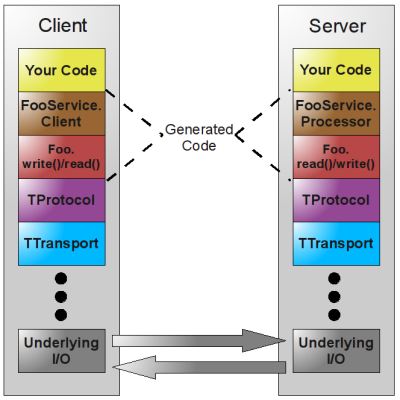
\includegraphics[width=0.25\textheight]{resources/chapter-2/thrift-arch.png}
        \caption{arsitektur Apache Thrift \parencite{prunicki_thrift}}
    \end{center}
\end{figure}

Secara bawaan, Apache Thrift mendukung beberapa transpor, protokol, dan server
\parencite{prunicki_thrift}. Dukungan-dukungan tersebut adalah
\begin{itemize}
    \item transpor (implementasi \texttt{TTransport}):
          \begin{itemize}
              \item \texttt{TSim\-ple\-FileTrans\-port}: menggunakan berkas,
              \item \texttt{TMe\-mo\-ry\-Trans\-port}: menggunakan memori,
              \item \texttt{T\-Sock\-et}: \textit{socket blocking},
              \item \texttt{TFramed\-Trans\-port}: pada server
                    \textit{nonblocking}, dan
              \item \texttt{T\-Z\-lib\-Trans\-port}: Melakukan kompresi dengan
                    zlib dan harus digunakan dengan trans\-por lain,
          \end{itemize}
    \item protokol (implementasi \texttt{TProtocol}):
          \begin{itemize}
              \item \texttt{TBinaryProtocol}: pesan dikirim dalam format
                    \textit{binary},
              \item \texttt{TCompactProtocol}: \texttt{TBinaryProtocol} yang
                    lebih \textit{compact},
              \item \texttt{TDenseProtocol}: \texttt{TCompactProtocol} yang
                    di\-hi\-lang\-kan \textit{me\-ta\-da\-ta}-nya, lalu ditambahkan
                    lagi oleh penerima,
              \item \texttt{TJsonProtocol}: pesan dikirim dalam format JSON,
              \item \texttt{TSimpleJsonProtocol}: \texttt{TJsonProtocol} tanpa
                    \textit{metadata}, cocok untuk bahasa \textit{scripting}, dan
              \item \texttt{TDebugProtocol}: format paling mudah dibaca manusia,
          \end{itemize}
    \item server (implementasi \texttt{TServer}):
          \begin{itemize}
              \item \texttt{TSimpleServer}: server \textit{single-threaded},
              \item \texttt{TThreadPoolServer}: server \textit{multi-threaded}
                    dengan \textit{blocking} I/O, dan
              \item \texttt{TNonBlockingServer}: server \textit{multi-threaded}
                    dengan \textit{non-blocking} I/O dan harus menggunakan
                    \texttt{TFramedTransport}.
          \end{itemize}
\end{itemize}

\subsection{Komunikasi Berorientasi Pesan}

Komunikasi berorientasi pesan adalah salah satu metode komunikasi pada sistem
terdistribusi. Metode ini utamanya bersifat
\textit{asynchronous}\footnote{Beberapa implementasi bisa \textit{synchronous}
    juga.}, artinya konsumen/klien tidak perlu \textit{blocking} ketika membuat
\textit{request}. Sifat \textit{asynchronous} ini merupakan alternatif untuk
serta cara berkomunikasi \textit{request/response} lainnya dan berguna ketika
konsumen tidak membutuhkan hasil pemrosesan pesan.

Implementasi untuk komunikasi berorientasi pesan yang akan dibahas adalah
protokol rosbridge dan pustaka ZeroMQ. Kedua protokol juga akan digunakan untuk
membuat jalur komunikasi antara server NVIDIA Pegasus dengan server simulator
CARLA.

\subsubsection{Rosbridge}

Rosbridge adalah protokol komunikasi yang menambahkan antarmuka pada komputer
dengan sistem operasi ROS. Antarmuka yang ditambahkan memungkinkan komunikasi
dengan pola \textit{publish/subscribe} dengan suatu topik ROS dalam format JSON.
Selain itu, antarmuka juga memungkinkan memanggil \textit{service} ROS
(komunikasi pola \textit{request/reply}).

Protokol rosbridge menggunakan format JSON untuk pesannya. Pesan yang valid
harus mengandung \textit{field} \texttt{"op"}. \textit{Field} tersebut digunakan
untuk menentukan jenis pesan. Pesan juga dapat mengandung \textit{field}
\texttt{"id"} yang digunakan sebagai penanda transaksi atau keterhubungan antara
beberapa pesan. Selain kedua \textit{field} tersebut, pesan rosbridge juga dapat
mengandung \textit{field} lainnya tergantung jenis \texttt{op}.

Secara arsitektur, rosbridge menggunakan WebSocket sebagai layanan
trans\-por\-nya. Artinya, pesan pada rosbridge pasti akan sampai dengan urutan
yang benar. Selain itu, pesan yang dikirim dapat berupa \textit{string} maupun
\textit{binary}. Pesan yang berupa \textit{string} adalah pesan dalam format
\textit{raw} JSON. Sedangkan dalam rupa \textit{binary}, rosbridge mendukung
kompresi dan \textit{encoding} dengan CBOR (\textit{concise binary object
    representation}) dan CBOR-\textit{raw}. Pesan CBOR harus didekompresi oleh
penerima menjadi \textit{raw} JSON.

Perbedaan antara CBOR dengan CBOR-\textit{raw} adalah format pesannya. Pada
CBOR-\textit{raw}, pesan dikirim dalam format serialisasi ROS. Keuntungan
menggunakan C\-B\-O\-R-\textit{raw} adalah peningkatan kinerja jika \textit{parsing}
hanya sebagian pesan, aplikasi dapat membaca berkas \texttt{bag}, atau
\textit{parsing} pesan ingin dilakukan seterlambat mungkin atau secara paralel.

\subsubsection{ZeroMQ}

ZeroMQ (\textit{zero message queue}) adalah sebuah pustaka yang merupakan
pe\-ning\-ka\-tan di atas \textit{socket} tradisional. ZeroMQ memberikan
fungsionalitas tambahan terhadap \textit{socket} dan mengabstraksi pembuatan
koneksi TCP dengan harapan memudahkan pengembangan aplikasi terdistribusi.
Fungsionalitas yang ditambahkan oleh ZeroMQ didasarkan pada pola-pola komunikasi
yang sering terjadi ketika menggunakan protokol TCP.

ZeroMQ memungkinkan komunikasi \textit{one-to-one} (seperti \textit{socket}
biasa), \textit{many-to-one} (\textit{socket} mendengarkan ke beberapa
\textit{port}), dan \textit{one-to-many}. Pola komunikasi yang didukung oleh
ZeroMQ adalah \textit{request-reply}, \textit{publish-subscribe}, dan
\textit{pipeline}. ZeroMQ juga memiliki sebuah antrian pesan (\textit{message
    queue}) sehingga pesan yang dikirimkan ke konsumen akan disimpan
sampai konsumen siap menerima pesan.

ZeroMQ berjalan di atas lapisan transpor ZMTP (ZeroMQ \textit{message transport
    protocol}). Semantik ZMTP memastikan pesan tidak akan diterima lebih dari 1 kali
oleh konsumen dan semua pesan akan diterima oleh konsumen dengan urutan yang
benar. Selain itu, \textit{frame} pesan yang diterima konsumen akan
di-\textit{queue} di memori penerima sampai semua \textit{frame} diterima.
Semantik ZMTP juga memastikan \textit{socket} dapat membuat dan menerima koneksi
serta \textit{socket} akan menyambungkan kembali jika koneksi terputus.

\section{Penelitian Terkait}
\blindtext